\documentclass[11pt,article,oneside]{article}

\usepackage[final,nonatbib]{neurips_2024}
\usepackage{booktabs}
\usepackage{algorithm}
\usepackage{algpseudocode}
\usepackage{multirow}
\usepackage{graphicx}
\usepackage{subcaption}

% Colors
\usepackage[dvipsnames]{xcolor}

% ===============
% Hyperlink setup
% ===============
\usepackage{xurl}
\usepackage[
    colorlinks,
    breaklinks=true,
    urlcolor=NavyBlue,
    citecolor=NavyBlue,
    linkcolor=NavyBlue,
    linktocpage,
]{hyperref}
\def\sectionautorefname{\S}
\def\subsectionautorefname{\S}

% Nicer monospace font
\usepackage{inconsolata}

% Using Palatino for text and math
\usepackage{newpxtext}
\usepackage{newpxmath}

% Improved typography
\usepackage{microtype}

% Bibliography setup
\usepackage[
    natbib,
    style=numeric-comp,
    sorting=none,
    doi=false,
    isbn=false,
    url=true,
    eprint=false,
    maxbibnames=10,
    hyperref
]{biblatex}
\addbibresource{bibliography.bib}
\renewcommand\bibfont{\small}
\newbibmacro{string+doiurlisbn}[1]{%
  \iffieldundef{doi}{%
    \iffieldundef{url}{%
      \iffieldundef{isbn}{%
        \iffieldundef{issn}{%
          #1%
        }{%
          \href{http://books.google.com/books?vid=ISSN\thefield{issn}}{#1}%
        }%
      }{%
        \href{http://books.google.com/books?vid=ISBN\thefield{isbn}}{#1}%
      }%
    }{%
      \href{\thefield{url}}{#1}%
    }%
  }{%
    \href{http://dx.doi.org/\thefield{doi}}{#1}%
  }%
}

\DeclareFieldFormat[article,book,incollection,inproceedings,data]{title}%
    {\usebibmacro{string+doiurlisbn}{#1}}

\DeclareFieldFormat*{url}{}
\DeclareFieldFormat[online]{url}{\mkbibacro{URL}\addcolon\space\url{#1}}

\DeclareFieldFormat[misc]{title}{\usebibmacro{string+doiurlisbn}{\mkbibemph{#1}}}


% Increase line spacing
\usepackage{setspace}
\setstretch{0.9} %

\title{Beyond Likes and Dislikes: Unveiling YouTube Comment Sentiment}
\author{%
    Jasdeep Singh Jhajj\\
    School of Information \\
    University of Arizona\\
    \texttt{jasdeepjhajj@arizona.edu}
}
\begin{document}
\maketitle

\section{Introduction}
The sudden and exponential growth of Youtube has led to the creation of active communities centered around content created by users. Comments on Youtube, specifically, provide a valuable source of information showcasing viewer thoughts, interaction frequency and general feelings towards a video. Examining these feelings can be extremely beneficial for creators, growing companies and researchers. \\

Understanding emotions from YouTube comments, which is a casual online text expression way is tricky because people might use some informal ways of text, emojis, or some common social media slang to express themselves. It is quite a tedious job if we have to build a team to manually analyze each and every comment, as every second thousands of videos get uploaded and also it can be prone to biasing and inconsistency in results. Using a mixture of machine learning techniques from natural language processing and supervised learning\citep{10.1007/978-981-13-6459-4_16} the model can handle the informality of the comments and even slangs being used in a phrase and analyze large volumes of comment data at once and categorize it into positive, negative, or neutral sentiment. One of the commendable work done in this field by \citet{Makhmudah}(2019), the authors used the support vector machine (SVM) algorithm for analysing sentiment of Tweets related to homosexuality in Indonesia, and achieved an accuracy around 99%.\\

This project focuses on building a model that can precisely categorize the sentiment of Youtube comments. Firstly, the Youtube Data API\citep{youtubeApiUsage} is used to gather comments from selected videos. As there will be use of casual language in Youtube comments, it can be tackled with proper data preprocessing to include text normalization, stop word removal, tokenization, and lemmatization\citep{Qi2023}. Studies like Khyani and B S (2021)\citep{khyaniArticle} delve into lemmatization and stemming, enriching our comprehension of text preprocessing in Natural Language Processing.As the data scraped will not be pre labeled to achieve data labeling I will then use Valence Aware Dictionary and Sentiment Reasoner(VADER)\citep{vaderUsage} to label the comments as positive, negative, or neutral for training purposes. Once trained, the evaluation parameter for the model can be based on accuracy, precision, and recall will be carefully assessed to evaluate its performance. \\

With a successfully trained sentiment analysis model, it can contribute to growth of small-scale brands, content creators to understand their target audience sentiment better, how their audience views their content, and eventually improve their content strategies. Hence, the project will be able to create a more meaningful and impactful online experience for creators and viewers. \\

\section{Methods}

\subsection{Data Handling}
\subsubsection{Data Collection}
The data collection for the Comments analysis is performed using the YouTube Data API v3\citep{youtubeApiUsage} using googleapiclient package. Google Cloud Console\citep{youtubeAPIKey} helps with the API key which was required to fetch the required information from the Youtube from a specific YouTube video ID, relevant comment data, including author name, comment text, publication time, and likes count were extracted from the API. The user is provided with interface to input a YouTube Video URL, from which the comments data is collected at runtime. The model trained and tested on the videos which have 9000 comments so that the model is properly trained without any kind of underfitting or overfitting.

\subsubsection{Data Preprocessing}
Data preprocessing is performed on the raw extracted comments to ensure data cleanliness and uniformity. The Youtube comments column in our dataset is cleaned by removing any non english character like special characters, numerical values, emojis/emoticons, converting to lowercase, and duplicate values and missing values are dropped appropriately. Finally, the comments are tokenized into separate words and lemmatization to make the analysis of feelings more efficient.

\subsubsection{Dataset Description}
The scraped dataset contains information about comments on a YouTube video. Here's a brief description of each column:

\textbf{Author\_Name}($<$str$>$): Usernames of individuals who posted the comments, starting with "@" followed by the username. \\
\textbf{Comment\_Text}($<$str$>$): It contains the actual text content of the comments posted by the users. \\
\textbf{Updated\_Time}($<$str Timestamp$>$): Timestamps indicating when the comments were posted in the format "YYYY-MM-DDTHH:MM:SSZ". \\
\textbf{Likes\_Count}($<$int$>$): Number of likes received by each comment.

\begin{table}[h]
\centering
\caption{Scrapped YouTube Comments Dataset}
\label{tab:yt_comments}
\begin{tabular}{cp{2.9cm}p{4.3cm}p{2.3cm}c}
\toprule
\textbf{Index} & \textbf{Author Name} & \textbf{Comment Text} & \textbf{Updated Time} & \textbf{Likes} \\
\midrule
1 & @spartanshivam2837 & Nyce & 2024-04-11T06:25:59Z & 0 \\
2 & @devsharma070 & Delious & 2024-04-11T04:49:49Z & 0 \\
3 & @abhi9800 & Wow.. best foods that I can think of. Great to... & 2024-04-11T04:41:35Z & 0 \\
4 & @Noobert & watched this while eating korma thinking about... & 2024-04-07T23:33:25Z & 0 \\
\bottomrule
\end{tabular}
\end{table}

\subsubsection{Data Labeling for Sentiment Analysis}
As the data extracted from Youtube API is not labelled, to analyse the sentiment we use the VADER\citep{vaderUsage} sentiment analysis tool from the NLTK library, function used to evaluate the comments polarity is \emph{polarity\_scores}. VADER  sentiment  analysis  relies  on  a  dictionary  that  maps  lexical  features  to emotion  intensities known  as  sentiment scores. The compound polarity score is calculated  by summing the valence scores of each word in the lexicon. The threshold based from the research of \citet{Hutto}(2015). If the compound score >= 0.05 then the text is labeled positive sentiment, value of compound score <= -0.05 is considered negative sentiment and others are neutral sentiment. By running this tool on every processed comment, we determine sentiment scores such as positive, negative, neutral, and compound. We categorize each comment's sentiment as good, negative, or neutral based on a compound score.

\subsection{Model \& Algorithm Description}
The model is created using scikit-learn's Pipeline class which includes two steps TfidfVectorizer and SVC(Support Vector Classifier). The first step of vectorizer, converts the text data using TF-IDF representation. It converts a collection of text documents into a matrix of TF-IDF features. The sentiment classification is done using the Support Vector Machine (SVM) algorithm\citep{SVMarticle}. The choice to use SVM was based on its ability to handle high-dimensional data and non-linear relationships useful for text classification. SVM finds an optimal hyperplane which can separate data points in a high-dimensional space into different classes. The transformation of input data to higher-dimensional space is achieved by kernel function, which can be of different type like linear, polynomial, radial-basis-function. The SVM model is trained on tokenized comments converted into numerical feature vectors, enabling it to recognize patterns in text and categorize comments into positive, negative, or neutral sentiments.

The dataset collected from Youtube comments is unbalanced in most of the cases, so one of the class becomes a minority class and the model is not able to learn that class properly, which leads to misclassifications in this case. So, to balance out all the classes a RandomOverSampler\citep{vaderUsage} is use to over-sample the minority class by picking samples randomly.
\begin{algorithm}
\caption{TrainSVM}
\begin{algorithmic}[1]
    \Procedure{TrainSVM}{$x_{\text{train}}, y_{\text{train}}, C_{\text{values}}, \text{kernel\_types}, num_{\text{folds}}$}
        \State Initialize empty list to store the performance metrics of each model
        \For{\textbf{each} $C$ \textbf{in} $C_{\text{values}}$}
            \For{\textbf{each} $\text{kernel\_type}$ \textbf{in} $\text{kernel\_types}$}
                \State Initialize SVM model with parameters $C$ and $\text{kernel\_type}$
                \State Initialize empty list to store performance metrics of each fold
                \For{$\text{fold} = 1$ \textbf{to} $num_{\text{folds}}$}
                    \State Split training data into training/validation sets using k-fold CV
                    \State Train the SVM model on training set $(x_{\text{train}}, y_{\text{train}})$
                    \State Evaluate the model on the validation set and calculate performance metrics
                    \State Add the performance metrics to the list of fold metrics
                \EndFor
                \State Calculate current model's average performance metrics over all folds
                \State Add the average performance metrics to the list of model metrics
            \EndFor
        \EndFor
        \State Find the model with the best average performance metrics
        \State Train the SVM model with the best hyperparameters on the entire training data
        \State \textbf{return} Trained SVM model with the best hyperparameters
    \EndProcedure
\end{algorithmic}
\end{algorithm}

\subsection{Evaluation Procedure}
The performance evaluation for the sentiment analysis model is performed by splitting the dataset into training, training a Support Vector Machine (SVM) classifier on the TF-IDF vectorized comments\citep{kilmen2022text} and testing sets and testing our model on unseen testing data then measuring metrics like, accuracy, precision, recall, and F1-score.Accuracy can be explained as a ratio of correctly predicted instances to the total instances. Precision is calculated as the ratio of predictions that should be positive  to the total positive predictions made. Recall is used to check the correctness of predicted positive instances out of all positives. F1-score combines the precision and recall into a single metric and is calculated as harmonic mean of precision and recall.

\begin{equation*}
\text{Precision} = \frac{\text{True Positives}}{\text{True Positives} + \text{False Positives}}
\end{equation*}

\begin{equation*}
\text{Accuracy} = \frac{\text{True Positives} + \text{True Negatives}}{\text{Total Instances}}
\end{equation*}

\begin{equation*}
\text{Recall} = \frac{\text{True Positives}}{\text{True Positives} + \text{False Negatives}}
\end{equation*}

\begin{equation*}
\text{F1 Score} = 2 \times \frac{\text{Precision} \times \text{Recall}}{\text{Precision} + \text{Recall}}
\end{equation*}

\subsection{Hyperparameter Tuning}
The accuracy of the Sentiment analysis SVM trained model can be maximized using the Hyperparameter tuning which requires optimizing the regularization parameter and the kernel coefficient. Grid search\citep{hyerparameterTuning} helps us search through a parameter grid, evaluating multiple possible combinations using cross-validation to find the optimal set of hyperparameters that maximizes the model's performance.

\section{Results}

\begin{figure}[H]
\centering
\begin{minipage}{0.48\textwidth}
Labeled Data Distribution After preprocessing the extracted comments from the API and labeling them, we have a distribution of sentiments in the labeled data as shown in the plot below which signifies distribution of Negative comments is 18.2\%, Neutral comments 35.2\% and rest of the comments are Positive comments 46.6\%. Sentiment distribution plot implies that for the given Youtube Video most of the comments belong to Positive sentiment, which is followed by Neutral and Negative sentiments.
\end{minipage}\hfill
\begin{minipage}{0.48\textwidth}
\centering
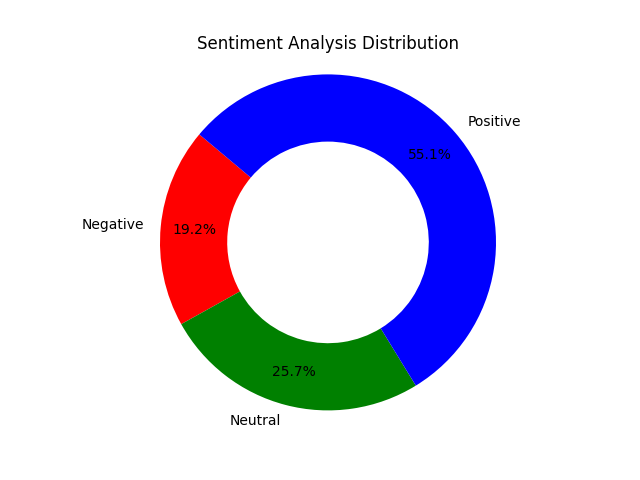
\includegraphics[width=\textwidth]{images/sentiment_pie_chart.png}
\caption{Sentiment Distribution}
\end{minipage}

\end{figure}

\textbf{Model Performance:}
The Support Vector Machine (SVM) model trained on the labeled data is evaluated on parameters like accuracy, precision\citep{precisionRecall}, F1-score\citep{f1scoreSupport}. The model achieved an accuracy of approximately 84.17\% on the test set which can be seen on the Result dashboard. This indicates that the well trained SVM model can effectively classify the sentiment of YouTube comments into one of the three categories: Negative, Neutral, or Positive with high reliability. \\

\begin{figure}[H]
    \centering
    \begin{subfigure}[b]{0.4\textwidth}
        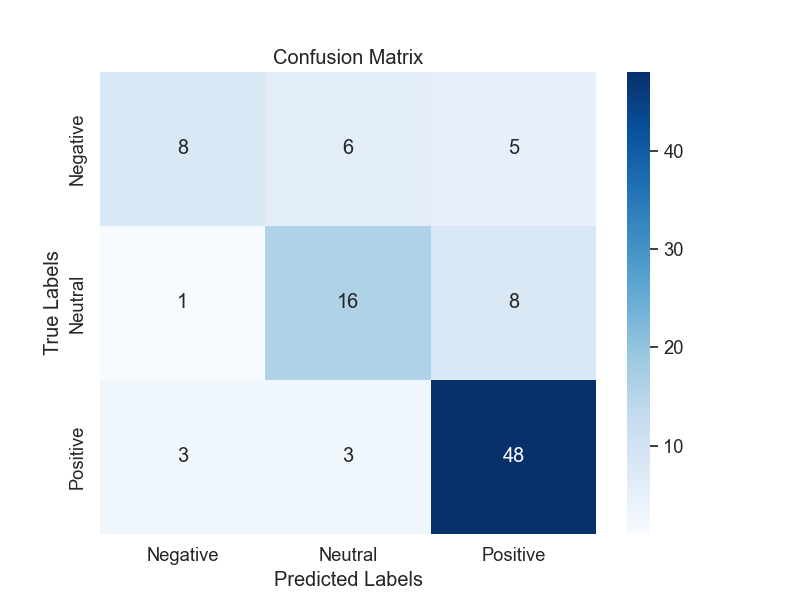
\includegraphics[width=\linewidth, height=4.9cm]{images/confusion_matrix.png}
        \caption{Confusion Matrix}
        \label{fig:subfig1}
    \end{subfigure}
    \begin{subfigure}[b]{0.4\textwidth}
        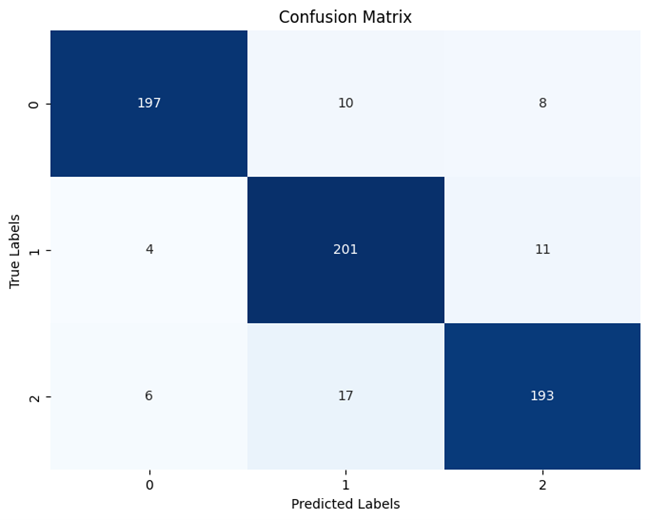
\includegraphics[width=\linewidth, height=4.9cm]{images/ConfusionMatrixafterBalance.png}
        \caption{Confusion Matrix}
        \label{fig:subfig1}
    \end{subfigure}
    \hfill
    \begin{subfigure}[b]{0.57\textwidth}
        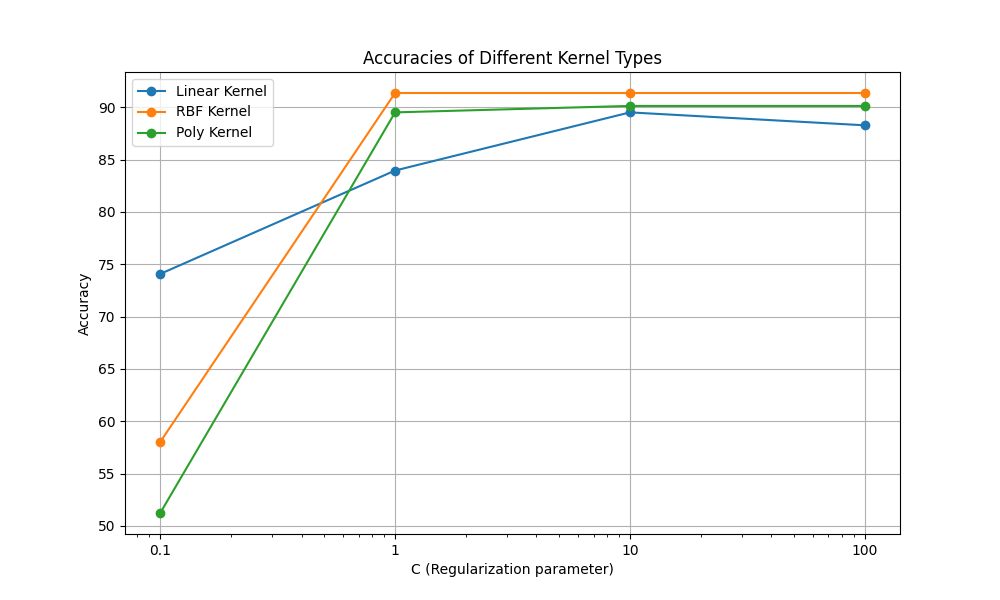
\includegraphics[width=\linewidth, height=4.9cm]{images/kernel_accuracies.png}
        \caption{Kernel Accuracies}
        \label{fig:comparison}
    \end{subfigure}

    \caption{Confusion Matrix and Different Kernel Accuracies}
    \label{fig:overall_label}
\end{figure}

\textbf{Confusion Matrix Analysis:}
The confusion matrix provides insights into the model's performance across different sentiment categories. It shows how many instances of each sentiment category were correctly or incorrectly classified. The diagonal element with higher values indicates correct classifications whereas Off-diagonal elements represent misclassifications.  From fig2(a), the comments that were correctly classified as Negative(True Negative) were 55 whereas there were some comments which were misclassified into Negative(21 Neutral comments and 7 Positive comments) which are considered False Positive for Negative Sentiment case. Similarly for the Neutral Sentiment we observe 150 comments were correctly classified as Neutral comment with a barely minimum False Negative in this case(2 Negative comments and 8 Positive comments). At last, for the Positive Sentiment, comments that are classified appropriately were 178 with a False Negative(10 Negative comments and 24 Neutral comments) being misclassified. Looking at figure 2(b), now that an oversampler is encorporated, the trained model will be learning equally about each class so it is verified by the diagonal elements being of almost equal range and the misclassification is reduced by large margin and diagonal elements have increased..
The confusion matrix plot provides a visual representation of the model's performance in terms of correct and incorrect classifications for each sentiment category.
It helps in identifying which sentiments are being confused with others and where the model's strengths and weaknesses lie. For instance if we look at the Negative Comment are misclassified by a significant amount like 21 Neutral comments and 7 Positive comments are classified as Negative. \\


\textbf{Accuracy for Different Kernel Types and Regularization Parameters:}
This plot shows accuracy for the SVM model when using different kernel types (linear, RBF, polynomial) across different values of the regularization parameter which is symbolized by C\citep{SVMparameterC} in this case. The regularization parameter (C) is plotted on x-axis and accuracy of each kernel type model plotted on y-axis. It helps to understand the relationship between regularization strength and model accuracy for three kernels. It helps in determining the optimal value of C that maximizes the model's performance.

\textbf{Classification report}

\begin{table}[h]
\centering
\caption{Classification Report for SVM model}
\label{tab:classification_report}
\begin{tabular}{p{3cm}cccc}
\toprule
\textbf{Class} & \textbf{Precision} & \textbf{Recall} & \textbf{F1-Score} & \textbf{Support} \\
\midrule
Negative & 0.70 & 0.76 & 0.73 & 94 \\
Neutral & 0.86 & 0.92 & 0.88 & 213 \\
Positive & 0.93 & 0.84 & 0.88 & 225 \\
\midrule
Macro Avg & 0.83 & 0.91 & 0.81 & 532 \\
Weighted Avg & 0.86 & 0.92 & 0.84 & 532 \\
\bottomrule
\end{tabular}
\end{table}

The classification report reveals the model's precision, recall, and F1-scores across negative, neutral, and positive sentiment categories. With an overall accuracy of 84\%, the model performs well in classifying comments,  Precision values of 0.70, 0.86, and 0.93 for negative, neutral, and positive sentiments, respectively, indicate the model's accuracy in classifying sentiments within each category. However, the classification for Negative comments seems to require an improvement as the precision of 70\% indicates the model includes many false positives. Recall is particularly high for Neutral comments (92\%), indicating the model effectively captures most actual Neutral comments. For Negative comments,  the recall of 76\% suggests there might be more false negatives compared to other classes which aligns with the discussion on Precision in classifying Negative comments. F1-score provides a more balanced perspective on the model's performance for each sentiment class. All F1-scores hover around 0.87, indicating a good equilibrium between precision and recall. The Support values, which represent the number of instances in each class, we observe 94 instances of negative sentiments, 213 instances of neutral sentiments, and 225 instances of positive sentiments.

\section{Discussion}

The sentiment analysis model based on Support Vector Machine (SVM) results in terms of accuracy and precision and F1-scores signify the performance in categorizing sentiments expressed in YouTube comments. Although the effectiveness of model, the confusion matrix highlights specific sentiment misclassifications, offering valuable insights for refining the model. The value of Precision denotes that the model is well trained and able to determine the sentiment with an accuracy of 84\%. Although the precision for Negative is not commendable, but for the Neutral and Positive ones it is quite effective. Observing the accuracy curve for various kernel types, we observe consistent performance with the linear kernel across different regularization parameter values (C). Linear kernel performs well in most of the cases with the accuracy peak at parameter value of 10. However, the RBF and polynomial kernels exhibit fluctuations in accuracy. The accuracy vs parameter plot serves as a deciding tool for fine-tuning the SVM model by identifying the optimal regularization parameter. In conclusion, the results and analysis display the effectiveness of the SVM model for the sentiment classification on YouTube comments with a possibility of additional improvements especially those targeting distinct misclassification patterns.

\newpage
\textbf{Results Dashboard}

\begin{figure}[H]
    \centering
    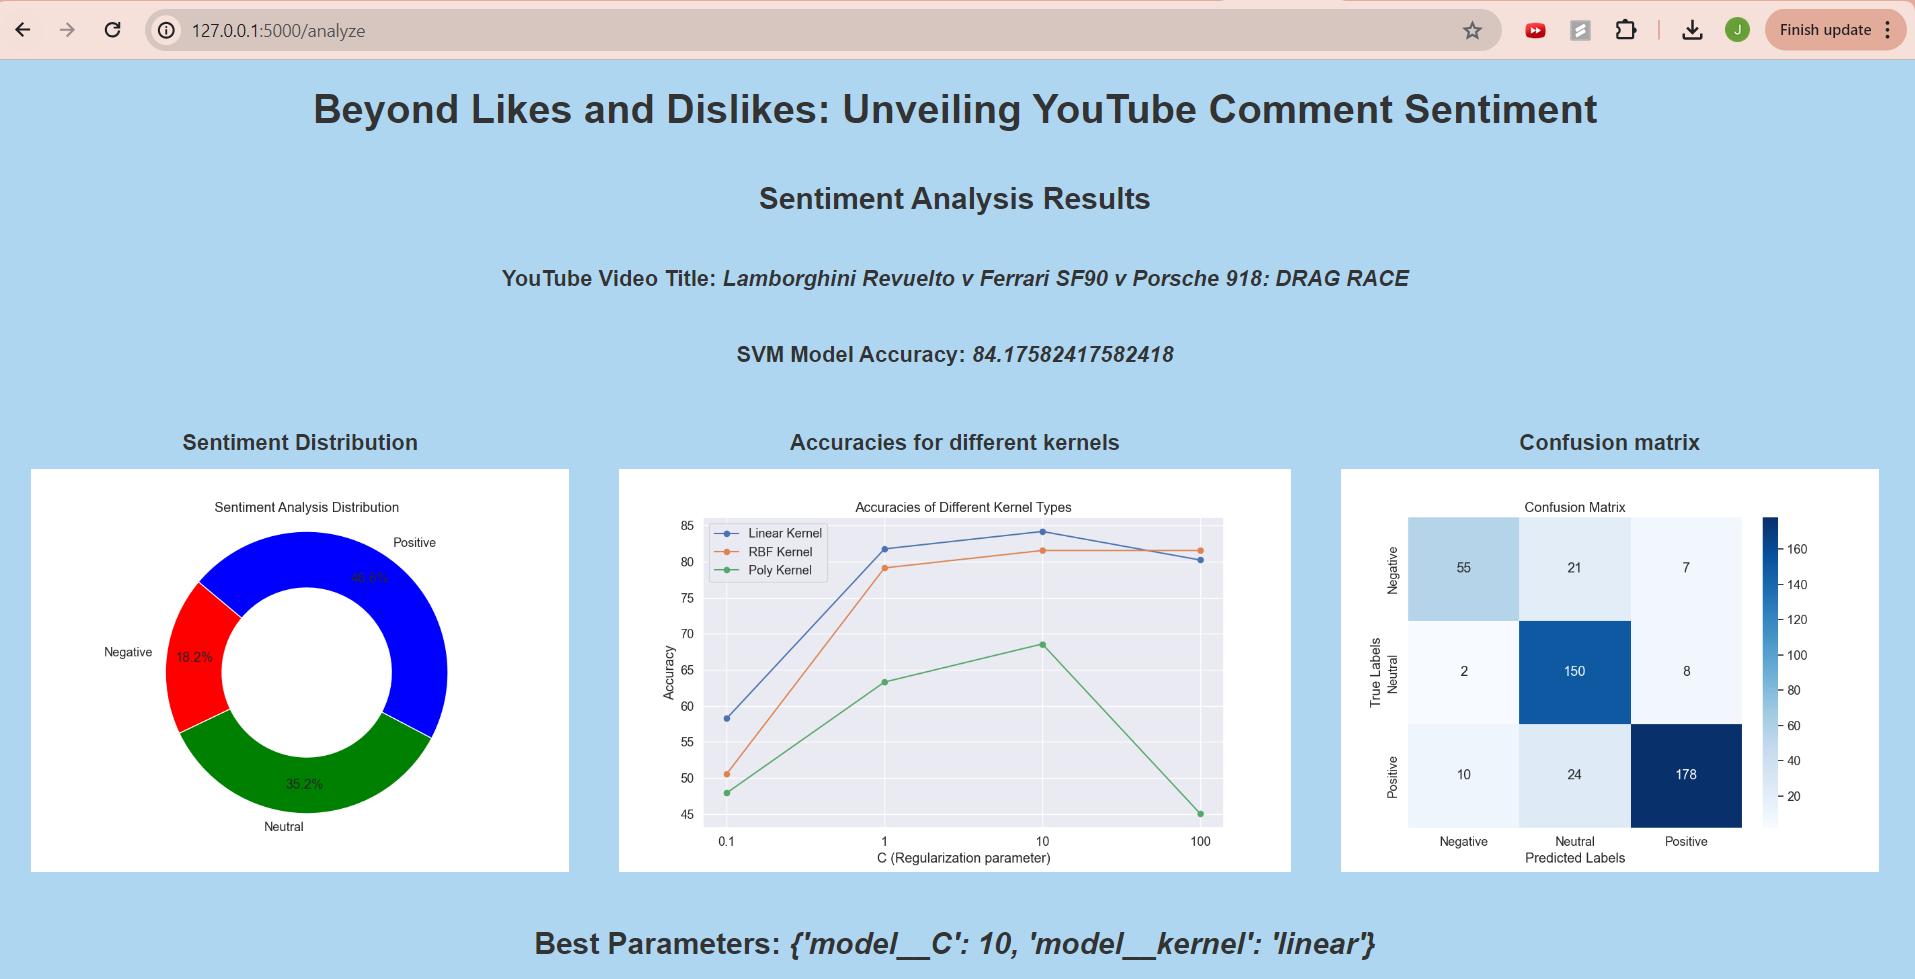
\includegraphics[width=0.9\textwidth]{images/yt_dashboard.PNG}
    \caption{Youtube Comment Analysis Results Dashboard}.
    \label{fig:results}
\end{figure}

\printbibliography

\end{document}
